			
			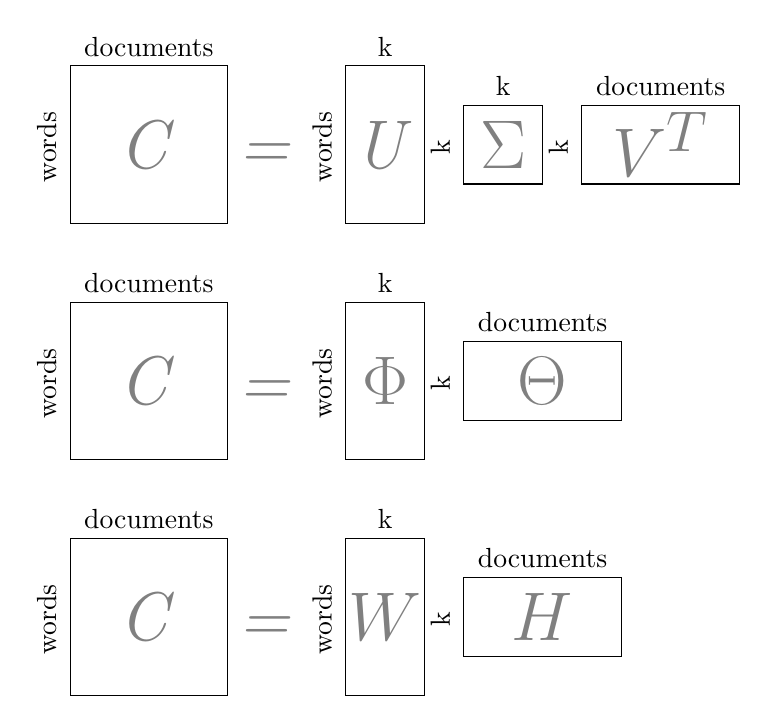
\begin{tikzpicture}
			
			% LSA
		 	\draw (0, 0) rectangle (2, 2);
		 	\node [above] at (1, 2) {documents};
		 	\node [right, rotate=90] at (-0.3, 0.4) {words};
		 	\node at (1, 1) {\Huge \color{gray} \textit{C}};
		 	\node at (2.5, 0.85) {\Huge \color{gray} \textit{=}};
		 	
		 	\draw (3.5, 0) rectangle (4.5, 2);
		 	\node [above] at (4, 2) {k};
		 	\node [right, rotate=90] at (3.2, 0.4) {words}; 
		 	\node at (4, 1) {\Huge \color{gray} \textit{U}};
		 	
		 	\draw (5, 0.5) rectangle (6, 1.5);
		 	\node [above] at (5.5, 1.5) {k};
		 	\node [right, rotate=90] at (4.7, 0.75) {k}; 
		 	\node at (5.5, 1) {\Huge \color{gray} \textit{$\Sigma$}};
		 	
		 	\draw (6.5, 0.5) rectangle (8.5, 1.5);
		 	\node [above] at (7.5, 1.5) {documents};
		 	\node [right, rotate=90] at (6.2, 0.75) {k}; 
		 	\node at (7.5, 1) {\Huge \color{gray} \textit{$V^T$}};
		 	
		 	
		 	% LDA
		 	
		 	\draw (0, -3) rectangle (2, -1);
		 	\node [above] at (1, -1) {documents};
		 	\node [right, rotate=90] at (-0.3, -2.6) {words};
		 	\node at (1, -2) {\Huge \color{gray} \textit{C}};
		 	\node at (2.5, -2.15) {\Huge \color{gray} \textit{=}};
		 	
		 	\draw (3.5, -3) rectangle (4.5, -1);
		 	\node [above] at (4, -1) {k};
		 	\node [right, rotate=90] at (3.2, -2.6) {words}; 
		 	\node at (4, -2) {\Huge \color{gray} $\Phi$};
		 	
		 	\draw (5, -2.5) rectangle (7, -1.5);
		 	\node [above] at (6, -1.5) {documents};
		 	\node [right, rotate=90] at (4.7, -2.25) {k}; 
		 	\node at (6, -2) {\Huge \color{gray} \textit{$\Theta$}};
		 	
		 	% NMF
		 	
		 	\draw (0, -6) rectangle (2, -4);
		 	\node [above] at (1, -4) {documents};
		 	\node [right, rotate=90] at (-0.3, -5.6) {words};
		 	\node at (1, -5) {\Huge \color{gray} \textit{C}};
		 	\node at (2.5, -5.15) {\Huge \color{gray} \textit{=}};
		 	
		 	\draw (3.5, -6) rectangle (4.5, -4);
		 	\node [above] at (4, -4) {k};
		 	\node [right, rotate=90] at (3.2, -5.6) {words}; 
		 	\node at (4, -5) {\Huge \color{gray} $W$};
		 	
		 	\draw (5, -5.5) rectangle (7, -4.5);
		 	\node [above] at (6, -4.5) {documents};
		 	\node [right, rotate=90] at (4.7, -5.25) {k}; 
		 	\node at (6, -5) {\Huge \color{gray} \textit{$H$}};
		 	\end{tikzpicture}
		 	
